%!TEX root = ../template.tex
%%%%%%%%%%%%%%%%%%%%%%%%%%%%%%%%%%%%%%%%%%%%%%%%%%%%%%%%%%%%%%%%%%%%
%% appendix1.tex
%% NOVA thesis document file
%%
%% Chapter with example of appendix with a short dummy text
%%%%%%%%%%%%%%%%%%%%%%%%%%%%%%%%%%%%%%%%%%%%%%%%%%%%%%%%%%%%%%%%%%%%

\typeout{NT FILE appendix1.tex}%

\chapter{Listings}
\label{app:listings}

\begin{listing}
\begin{minted}
[
frame=lines,
linenos,
fontsize=\scriptsize
]
{cpp}
marrow_function
idx_t binary_search(std::size_t tid, std::size_t frontier_size, std::size_t* degrees_scan) {
    int frontier_vertex_n = -1;
    int low = 0, high = frontier_size - 1;
    while (frontier_vertex_n == -1 && low <= high) {
        int mid = (low + high) / 2;
        if (tid < degrees_scan[mid] && (mid==0 || tid >= degrees_scan[mid-1]))
            frontier_vertex_n = mid;
        else if (tid < degrees_scan[mid])
            high = mid - 1;
        else
            low = mid + 1;
    }
    return frontier_vertex_n;
}
\end{minted}
\center
\caption{Graph Bal Binary Search.}
\label{lst:binary_search}
\end{listing}

\begin{listing}
\begin{minted}
[
frame=lines,
linenos,
fontsize=\scriptsize
]
{cpp}
template<typename vertex_attributes, typename edge_attributes, 
  typename on_intersection_fun, typename... on_intersection_arguments>
__device__
int segmented_intersection(
        graph_bal_t<vertex_attributes, edge_attributes> &graph,
        vertex<vertex_attributes>& vertex_a,
        vertex<vertex_attributes>& vertex_b,
        on_intersection_fun on_intersection,
        on_intersection_arguments&... on_intersection_args) {

    using Vertex = vertex<vertex_attributes>;
    using Edge  = edge<edge_attributes>;

    int nintersections = 0;
    int degree_a = graph.vertices[vertex_a.idx].degree;
    int degree_b = graph.vertices[vertex_b.idx].degree;
    int block_index_a = graph.vertices[vertex_a.idx].adjacency_list;
    int block_index_b = graph.vertices[vertex_b.idx].adjacency_list;
    int offset_a = 0;
    int offset_b = 0;
    int index_a = 0;
    int index_b = 0;

    while (index_a < degree_a && index_b < degree_b) {

        int edges_index_a = block_index_a * graph.block_size + offset_a;
        int edges_index_b = block_index_b * graph.block_size + offset_b;
        Vertex& neighbor_a = graph.vertices[graph.edges[edges_index_a].dst];
        Vertex& neighbor_b = graph.vertices[graph.edges[edges_index_b].dst];

        if (neighbor_a.idx == neighbor_b.idx) {
            nintersections++;
            on_intersection(vertex_a, vertex_b, neighbor_a, on_intersection_args...);
            index_a++;
            offset_a++;
            index_b++;
            offset_b++;
        }
        else if (neighbor_a.idx > neighbor_b.idx) {
            index_b++;
            offset_b++;
        }
        else {
            index_a++;
            offset_a++;
        }

        if (offset_a >= graph.block_size) {
            offset_a = 0;
            block_index_a = graph.block_links[block_index_a];
        }
        if (offset_b >= graph.block_size) {
            offset_b = 0;
            block_index_b = graph.block_links[block_index_b];
        }
    }

    return nintersections;
}
\end{minted}
\center
\caption{Segmented Intersection.}
\label{lst:segmented_intersection}
\end{listing}

\begin{listing}[H]
\begin{minted}
[
frame=lines,
linenos,
fontsize=\scriptsize
]
{cpp}
template <typename vertex_attributes, typename edge_attributes, std::size_t block_size>
struct graph_bal_sort_adjacency_list_fun {
    using Block = array<edge<edge_attributes>, block_size>;
    vertex<vertex_attributes>& src_vertex;
    vector<Block>& blocks;
    vector<idx_t>& block_links;

    graph_bal_sort_adjacency_list_fun(vertex<vertex_attributes>& src_vertex, 
      vector<Block>& blocks, vector<idx_t>& block_links) :
        src_vertex(src_vertex), blocks(blocks), block_links(block_links) {
    }

    void operator()() {
        quick_sort(0, src_vertex.degree-1);
    }

    void quick_sort(int start, int end) {

        if (start >= end)
            return;

        int p = partition(start, end);
        quick_sort(start, p - 1);
        quick_sort(p + 1, end);
    }

    edge<edge_attributes>& get(int i) {
        int block_n = i/block_size;
        int offset = i%block_size;
        int block_index = src_vertex.adjacency_list;
        for(int j = 0; j < block_n; j++)
            block_index = block_links.read(block_index);
        Block& block = blocks.read(block_index);
        return block.read(offset);
    }

    void swap(edge<edge_attributes> *a, edge<edge_attributes> *b) {
        edge<edge_attributes> t = *a;
        *a = *b;
        *b = t;
    }

    int partition(int low, int high) {
        int pivot = get(high).dst;
        int i = (low - 1);
        for (int j = low; j < high; j++) {
            if (get(j).dst <= pivot) {
                i++;
                swap(&get(i), &get(j));
            }
        }
        swap(&get(i + 1), &get(high));
        return (i + 1);
    }
};

template <typename vertex_attributes, typename edge_attributes, std::size_t block_size>
void graph_bal_sort_adjacency_list(/*...*/) {

    graph_bal_sort_adjacency_list_fun(/*...*/)();
}
\end{minted}
\center
\caption{Sort Adjacency List.}
\label{lst:sort_adjacency_list}
\end{listing}

\begin{listing}[H]
\begin{minted}
[
frame=lines,
linenos,
fontsize=\scriptsize
]
{cpp}
struct graph_bal_frontierless_advance_fun : function_with_coordinates</*...*/> {

    template<typename vertex_attributes, 
      typename edge_attributes, typename compute_fun, typename... compute_args>
    marrow_function
    void operator()(coordinate_t* coordinate,
                    idx_t *frontier,
                    vertex<vertex_attributes> *vertices,
                    edge<edge_attributes> *edges,
                    std::size_t block_size,
                    idx_t *block_links,
                    std::size_t frontier_size,
                    compute_fun &compute,
                    compute_args &... comp_args) {

        using Vertex = vertex<vertex_attributes>;
        using Edge = edge<edge_attributes>;
        using Graph = graph_bal_t<vertex_attributes, edge_attributes>;

        const std::size_t tid = coordinate[0];
        idx_t vertex_idx = frontier[tid];
        Vertex &vertex = vertices[vertex_idx];

        int neighbour_n = 0;
        for (idx_t block_idx = vertex.adjacency_list;
             block_idx != -1 && neighbour_n < vertex.degree; block_idx = block_links[block_idx]) {

            for (std::size_t block_offset = 0;
                 block_offset < block_size && neighbour_n < vertex.degree; block_offset++) {

                Edge _edge = edges[block_idx * block_size + block_offset];

                if constexpr (std::is_invocable<decltype(compute), 
                  Graph &, Vertex &, Vertex &, Edge &, compute_args &...>::value) {

                    Graph graph = {
                            .block_size = block_size,
                            .vertices = vertices,
                            .edges = edges,
                            .block_links = block_links
                    };

                    compute(graph, vertex, vertices[_edge.dst], _edge, comp_args...);
                } else {
                    compute(vertex, vertices[_edge.dst], _edge, comp_args...);
                }

                neighbour_n++;
            }
        }
    }
};
\end{minted}
\center
\caption{Graph Bal Unbalanced Frontierless Advance Marrow Function.}
\label{lst:graph_bal_unbalanced_frontierless_advance_marrow_function}
\end{listing}

\begin{listing}%[t]
\begin{minted}
[
frame=lines,
linenos,
fontsize=\scriptsize
]
{cpp}
template <typename vertex_attributes, typename edge_attributes>
class graph {

    using Vertex = vertex<vertex_attributes>;
    using Edge = edge<edge_attributes>;
public:
    virtual idx_t add_vertex(vertex_attributes attributes) = 0;
    virtual bool remove_vertex(idx_t idx) = 0;
    virtual bool add_edge(idx_t src, idx_t dst, edge_attributes attributes) = 0;
    virtual bool add_edge_batch(edge_insertion_batch<edge_attributes>& batch) = 0;
    virtual bool remove_edge(idx_t src, idx_t dst) = 0;
    virtual bool remove_edge_batch(edge_deletion_batch<edge_attributes>& batch) = 0;
    virtual bool edit_edge(idx_t src, idx_t dst, idx_t new_dst) = 0;
    virtual vector<idx_t> get_connection(idx_t idx) = 0;
    virtual std::size_t get_degree(idx_t idx) = 0;
    virtual std::size_t get_number_of_vertex() = 0;
    virtual std::size_t get_number_of_edges() = 0;
    virtual void sort() = 0;

    template <bool return_frontier = true, bool balanced = true>
    template <typename compute_fun, typename... compute_args>
    auto advance(vector<idx_t>& frontier, compute_fun& cfun, compute_args&... cargs);
    
    template <typename filter_fun, typename... filter_args>
    auto filter(vector<idx_t> &frontier, filter_fun& ffun, filter_args&... fargs);
};
\end{minted}
\center
\caption{Graph interface.}
\label{lst:graph_interface_complete}
\end{listing}

%\section{CUDA}

% \begin{listing}[H]
% \begin{minted}[frame=single, fontsize=\scriptsize]{cpp}
% #define N 2048
% #define THREADS_PER_BLOCK 512

% __global__
% void add(int* res, int* b, int* c, int n)
% {
%     int index = threadIdx.x + blockIdx.x*blockDim.x;

%     if(index < n)
%         res[index] = b[index] + c[index];
% }

% int main()
% {
%     int *res, *b, *c;
%     int *d_res, *d_b, *d_c; // Device data
%     int size = N * sizeof(int);

%     // Allocate and init host data
%     b = (int*)malloc(size);
%     c = (int*)malloc(size);
%     res = (int*)malloc(size);
%     init_data(b, c, N);

%     // Allocate device data
%     cudaMalloc((void**)&d_b, size);
%     cudaMalloc((void**)&d_c, size);
%     cudaMalloc((void**)&d_res, size);

%     // Copy data from host to device
%     cudaMemcpy(d_b, b, size, cudaMemcpyHostToDevice);
%     cudaMemcpy(d_c, c, size, cudaMemcpyHostToDevice);

%     // Specify grid and envoke kernel
%     // ceiling
%     long nb = (N+THREADS_PER_BLOCK-1)/THREADS_PER_BLOCK;
%     add<<<nb, THREADS_PER_BLOCK>>>(d_res, d_b, d_c, N);

%     // Copy result data from device to host
%     cudaMemcpy(res, d_res, size, cudaMemcpyDeviceToHost);

%     // Deallocate memory
%     cudaFree(d_b); cudaFree(d_c); cudaFree(d_res);
%     free(b); free(c); free(res);
% }
% \end{minted}
% \center
% \title{CUDA add vectors main function}
% \label{lst:cuda-add-vecs-main}
% \end{listing}

% \begin{figure}
% \label{fig:sm}
%   \centering
%     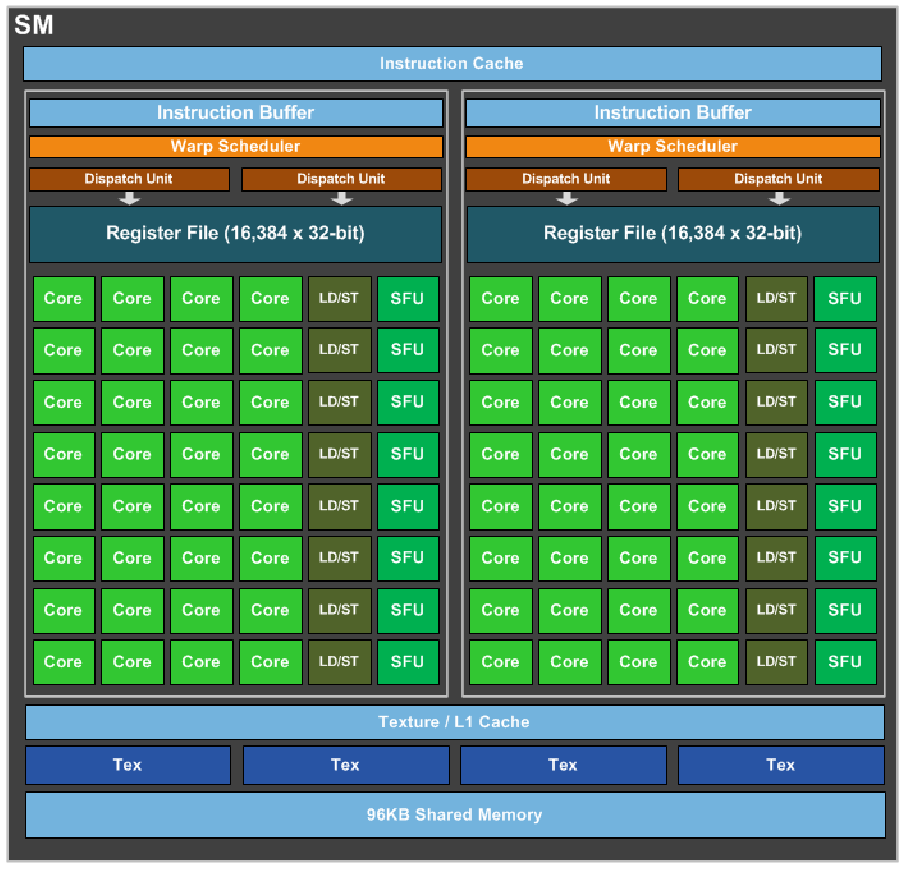
\includegraphics[width=0.65\textwidth]{Chapters/Figures/Images/sm_2.png}
%     \caption{Pascal Stream Multiprocessor}
% \end{figure}

%\lipsum[1-5]
